\chapter{Coleta de Dados}
\label{cap:coleta-dados}

Para esta pesquisa, será utilizada uma base de dados extraídos do \gls{NPM}. Esta base contém informações sobre todos os pacotes hospedados no \gls{NPM} até jun/2017, totalizando \textit{366,629} pacotes. Para cada pacote, há informações sobre cada uma de suas \textit{releases}. A Tabela \ref{tab:database} contém as informações para o pacote \textit{streamme}\footnote{https://npmjs.org/package/streamme}:

\begin{itemize}
    \item \textit{name}: o nome do pacote cliente;
    \item \textit{version}: as versões de cada \textit{release} do pacote cliente;
    \item \textit{timestamp}/\textit{prev\_timestamp}: contêm os \textit{timestamp} relacionados àquela determinada \textit{release};
    \item \textit{prov\_name}: os nomes dos provedores daquela \textit{release};
    \item \textit{prov\_vers}: contém, no momento da \textit{release} do cliente, a última versão que o cliente aceitava dos provedores; e
    \item \textit{prov\_vers\_chng}: informa o tipo de atualização que os provedores realizaram desde a última \textit{release} do cliente:
    \begin{itemize}
        \item se vazio: o provedor foi adicionado nesta \textit{release};
        \item \textit{steady}: a versão aceita do provedor não foi alterada desde a última \textit{release} do cliente, ou seja, o provedor não publicou nenhuma \textit{release} aceita pelo cliente; e
        \item \textit{upgrade}: o provedor publicou uma \textit{release} desde a última \textit{release} do cliente, ou seja, o cliente aceita uma nova \textit{release} do provedor.
    \end{itemize}
\end{itemize}{}

\begin{table}[!h]
    \scalebox{0.72}{
        \begin{tabular}{|c|c|c|c|c|c|c|c|}
            \hline
            name & version & timestamp & prev\_timestamp & prov\_name & prov\_vers & prov\_vers\_chng \\ \hline
            streamme & 0.0.0 & 2016-03-30T02:52:15.107Z &  &  &  &  \\ \hline
            streamme & 0.0.1 & 2016-04-22T01:13:50.263Z & 2016-03-30T02:52:15.107Z & util & 0.10.3 &  \\ \hline
            streamme & 0.0.1 & 2016-04-22T01:13:50.263Z & 2016-03-30T02:52:15.107Z & sync-request & 3.0.0 &  \\ \hline
            streamme & 0.1.0 & 2016-04-25T20:15:47.753Z & 2016-04-22T01:13:50.263Z & util & 0.10.3 & steady \\ \hline
            streamme & 0.1.0 & 2016-04-25T20:15:47.753Z & 2016-04-22T01:13:50.263Z & sync-request & 3.0.1 & upgrade \\ \hline
        \end{tabular}
    }
    \caption{Formato da base de dados para cada pacote do NPM}
    \label{tab:database}
\end{table}

A quantidade da amostra para o estudo é de 384 pacotes, com base em um cálculo amostral\footnote{https://pt.surveymonkey.com/mp/sample-size-calculator/} com 95\% de confiança e 5\% de margem de erro. Dos \textit{366K} de pacotes, a amostra de 384 pacotes foi recuperada sorteando um número no intervalo \textit{0-366,629}. Do pacote sorteado, foi recuperado o seu \textit{package.json} e verificado se o pacote cumpre quatro requisitos: possui mais de 1 provedor --  se não houver provedores, não há possibilidades do pacote sofrer \textit{breaking changes}; possui pelo menos a última \textit{release} com \textit{script} de teste não vazio e diferente do \textit{script} padrão de teste do \gls{NPM}: \textit{Error: no test specified}; possui a \textit{url} do repositório do pacote; e o repositório do pacote precisa existir -- será esperado de uma requisição \Gls{HTTP} para o repositório o código \textit{200} indicando sua existência. A Figura \ref{fig:package_json} exemplifica as informações pertinentes no \textit{package.json} do pacote \textit{raven@0.1.0}\footnote{http://registry.npmjs.org/raven}.

\begin{figure}
    \centering
    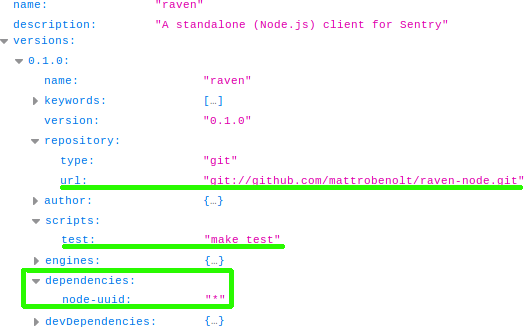
\includegraphics[scale=0.7]{figuras/package_json.png}
    \caption{Informações que serão recuperadas do \textit{package.json} para validar um pacote}
    \label{fig:package_json}
\end{figure}{}

Ao todo, foram sorteados e recuperados 404 pacotes para o estudo. Destes 404, em 20 pacotes não foi possível executar o comando \textit{npm install}/\textit{npm test} para nenhuma de suas versões. Isso porque estes pacotes apresentaram algum tipo de erro que impossibilitou a execução. Destes 20 pacotes, 15 não possuía algum dos arquivos necessários para os testes; 4 haviam listados alguns dos arquivos no \textit{.gitignore}, mas que eram necessários para a execução; e um pacote foi considerado como um \textit{toy package}, ou seja, não era um projeto real, apenas um repositório no qual o desenvolvedor, provavelmente, criou para testar o \gls{NPM}. Então, outros 20 pacotes tiveram que ser substituídos em um novo sorteio, totalizando 384 pacotes utilizados no estudo. A Figura \ref{fig:database} apresenta a distribuição de provedores e de \textit{releases}, na qual os \textit{boxplots} em azul -- dois primeiros -- representam a amostra e os \textit{boxplots} em vermelho -- dois últimos -- representam a base de dados.

\begin{figure}
    \centering
    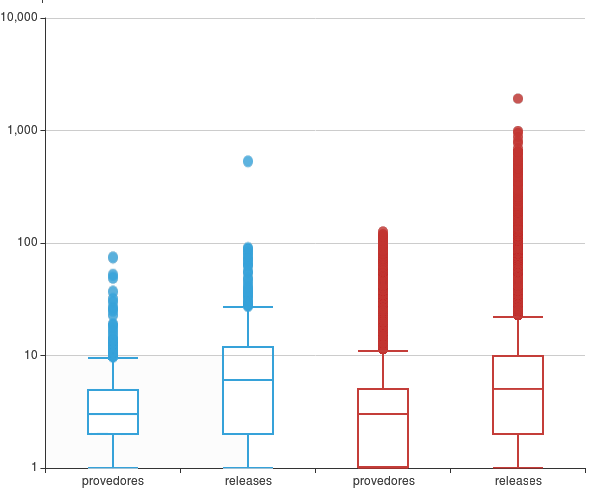
\includegraphics[scale=0.6]{figuras/data_box_plot_pt.png}
    \caption{Distribuição de provedores e \textit{releases} da amostra e da base, respectivamente}
    \label{fig:database}
\end{figure}{}